%!TEX root = ../Peerbox.tex
Peer-to-peer systems have become  popular  in social, academic and commercial domains. These systems use networks in which each computer can act as a client or server for other computers without the need of a central server. One of the early driving forces behind peer-to-peer concept is that there are many PC's at home and offices that lie idle for large chunks of time. These resources can be leveraged for content sharing. This report has been created during the Distributed Systems course 12/13 at the University of Groningen.

In this report, we present the design and implementation of a peer-to-peer file sharing system called Peerbox. Peerbox is mainly targeted for university students who want to share their work among their group. This system proves helpful in sharing files during small projects. It is intended for small groups with an average size of four members. Peerbox is able to provide characteristics like scalability, performance and heterogeneity. However, there are still open issues like security, mobile transparency, location transparency and replication that need to be addressed in the future. 

Section 1 describes the general idea and requirements  of Peerbox. Section 2 compares state-of-the-art peer-to-peer file sysytem with each other and puts them into perspective. Section 3 discusses potential scenarios and assumptions about the Peerbox domain.  Section 4 presents the overall architecture, design and implementation of the system. Finally, Section 5  discusses the results by examining typical characteristics of distributed file systems. 

\subsection{Idea}

Christian, Divya and Spyros are students who work on a project for their Cloud Computing course. Typically they meet every second day to synchronize their work and discuss the further progress of the project. These meetings often require to share files with each other. However, there may be some situations where internet is not available. Nevertheless, the students need to work effectively by sharing their work - this means that they should be able to access files that are stored on another computer in an easy and straight-forward manner. This can be accomplished by combining the computers in a \gls{acr:vfs} that automatically adds files in a peer-to-peer scheme. Hence, the VFS would  detect new peers and show their files, so that they can be accessed by the group members.

Implementing the proposed solution, would  enable them to work across network boundaries without setting up complex shared folders, by creating a flexible file system structure. In this way, the students would not need to transmit ownership of a file because  files are stored locally on their computers. Thus, File sharing will be possible with minimal configuration. Figure~\ref{fig:idea} illustrates the general idea of Peerbox.

 
\begin{figure}[H]
\begin{center}
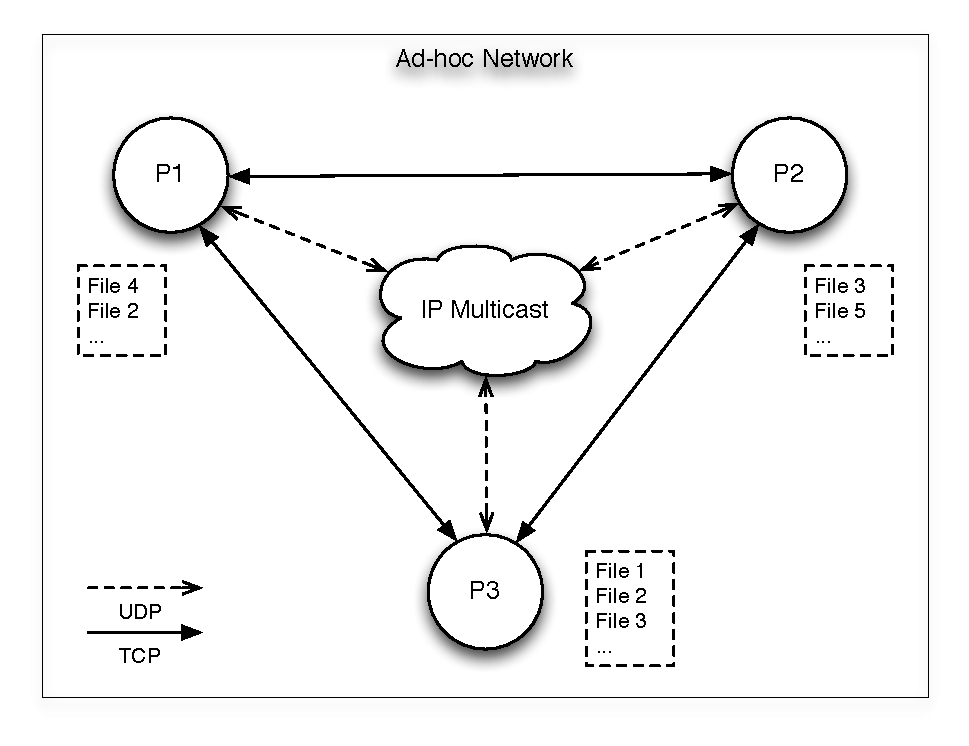
\includegraphics[height=3.2in]{figures/idea.pdf}
\caption{The high level idea of Peerbox}
\label{fig:idea}
\end{center}
\end{figure}



\subsection{Context}
%manni
The main goal of the Peerbox system is to enable file sharing among different peers. Here, the process of multicasting is used where a set of data packets are transmitted to  multiple hosts who have joined the multicast group simultaneously. 

After joining the group, the peer can request the list of files, create files, update the files as well as delete files.


\clearpage
\section{State of the Art}
%spyros

During the last decade, various peer-to-peer file systems were introduced. Most of them share common properties like availability, sharing, safety and decentralization. However, some more advanced peer-to-peer file systems offer important properties like synchronization and conflict detection. This section provides the state of the art in peer-to-peer file systems.

\begin{description}
	\item[Pastis]\-\\
	Pastis \cite{Busca:2005gt} is a decentralized multi-user read-write peer-to-peer file system. Every file is described by
a modifiable inode-like structure which contains the addresses of the immutable blocks in which the file contents are stored.

All the data is stored using the Past \gls{acr:dht}, which has been modified in order to reduce the number of network messages it generates, thus optimizing replica retrieval. Pastis is known for its simplicity, high scalability, fault tolerance and locality properties of its underlying storage layer.

	\item[Ivy]\-\\
	Ivy \cite{Muthitacharoen:2002iv} is a multi-user read and write peer-to-peer file system. It has no centralized or dedicated components. It provides useful integrity properties without requiring users to fully trust either the underlying peer-to-peer storage or other users of the file system.
	
	One of its important properties is that with a special arrangement between logs and the modifications of participants, it maintains meta-data consistency without locking. Ivy provides semantics like \gls{acr:nfs} and is able of detecting conflicting modifications. Performance measurements show that Ivy is two to three time slower than \gls{acr:nfs}.
	\item[ColonyFs]\-\\
	ColonyFS \cite{Colony:2009fs} is a distributed file system which emphasizes anonymity, security and dependability over a peer to peer network. This system implements a technique called \gls{acr:frs} and uses an optimization algorithm inspired by the movement of ants. The aim of the project is to produce an implementation of these techniques for the specific requirements of a dynamic peer-to-peer network where participants can join and leave at will.
	\item[Infinit]\-\\
	Infinit\footnote{http://en.wikipedia.org/wiki/Infinit} is a peer-to-peer file system which allows users to store, access and share files in a safe and collaborative way. It also allows the virtualization of decentralized storage space as one coherent drive. Infinit ensures reliability by dynamically replicating the data so that devices can crash without incurring data loss. It also ensures privacy by access control mechanisms.
	
	Furthermore, it is known for ensuring synchronization by distributing files and directories throughout the network's infrastructure and update them in real time. Some additional properties of Infinit are sharing, transparency, security, anonymity, and availability.
	\item[Darknet]\-\\
	Darknet \cite{Ledung:2010wq} is private peer-to-peer file system which aims to provide safe, fast, and scalable file sharing without constraining the users in this aspect. It utilizes a decentralized peer-to-peer network overlay by creating a prototype with extreme programming as methodology. To maximize the freedom of users the network is accessed through a virtual file-system interface.
\end{description}
